\section{Security Context}
\label{sec:securitycontext}

\begin{figure}
    \centering
        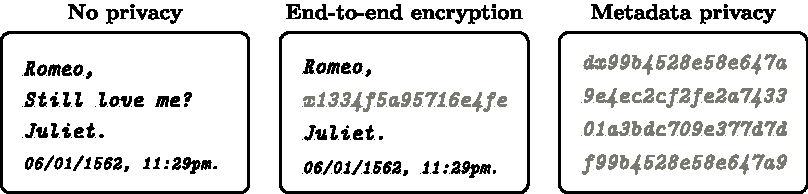
\includegraphics[width=\textwidth]{metadata-privacy.pdf}
\caption{The view of a powerful adversary in three different threat models. With end-to-end encryption, the adversary can still see the metadata.}
\label{fig:metadataprivacy}
\end{figure}



In this section, we describe what our system achieves beyond end-to-end encrypted messaging applications like Signal and Wickr.

Signal is great. It is end-to-end encrypted, open source, and run by a trustworthy group. Unfortunately, if their servers are hacked, one of their employees bribed, or you are attacked by a network-level powerful actor, there is nothing Signal can guarantee. \xxx[stzh]{I do not think so. The point of E2E encryption is to guarantee content security when the server gets compromised.}

Furthermore, even with a secure server, it leaks metadata.  Using timing attacks, an adversary can figure out when, where and with whom you are talking. 

\subsection{Desired Properties}

1. \textbf{Metadata Protection}: All contents and metadata of a conversation are only visible to the users involved in the conversation. Even with all servers compromised, an adversary should not be able to find out whether two users are engaging in conversation.

An especially challenging case is metadata protection during trust establishment. This happens when two users wish to add each other as friends for the first time. This feature is not supported even by Addra or Pung. We outline our solution in \cref{sec:trustestablishment}, which offers users a variety of options to establishing trust.

2. \textbf{Resistance to MITM attacks}: We use PIR and end-to-end encryption to ensure no man-in-the-middle(MITM) can access metadata associated with any conversation of the user.

3. \textbf{Resistance to DoS attacks}: Denial of Service(DoS) attacks are unavoidable if the adversary controls all our servers. In the case of a server-controlling adversary, we do not guarantee liveliness of our service, but continue to guarantee metadata security. We also defend against DoS attacks launched by an end-user with no access to the servers.

4. \textbf{Reasonable Load on Client and Server}: Since PIR is expensive, we design our system to minimize load on the client and server without compromising security. We use the most efficient PIR algorithms known on the server. We also give users the option to adjust client side load to suit their upload and download bandwidth.

\subsection{Threat Model}
\label{subsec:threatmodel}


We plan to achieve our goals in the presence of strong adversaries, whose capabilities we define in this section. Our belief in no needless trust means that our threat model is as extensive as possible.

%\begin{table*}[t]
%\centering
%another version below
%\begin{tabular}{||c c c c c c||} 
% \hline
%  Attacker compromises $\cdots$ & Anysphere & Signal & Skiff & Wickr & Onion  \\
% \hline
% Attacker listens on the internet & \checkmark & \checkmark & \checkmark & \checkmark \\ 
% \hline
% Attacker compromises & \checkmark & & & \checkmark & \checkmark \\
% \hline
% Skiff & \checkmark &  &  & & \checkmark\\
% \hline
% Wickr & \checkmark & & & \checkmark & \checkmark\\
% \hline
% Onion & \checkmark & *\footnote{\label{onion}Only guaranteed for non-global adversary} & &\checkmark&\checkmark\\
% \hline
%\end{tabular}
%\caption{Comparing when}
%\end{table*}

% \xxx{add an illustration of a walled garden, with the walls containing only your computer and your friends' computers} 

%Touch on: server, friends, client-side computer, etc.

\textbf{1. The attacker may compromise all servers.} To achieve privacy, we do not put any trust in the server. Our threat model assumes a global adversary who has full control over all servers, and can observe and manipulate all network traffic. This is similar to other anonymous communication schemes based on private information retrieval (for example \cite{ahmad2021addra}, \textsection 2.2), but stronger than most other anonymous communication schemes (e.g. Tor \cite{dingledine2004tor} and Nym \cite{piotrowska2017loopix}, which require partial trust in the servers).

\textbf{2. The attacker may control the entire internet.} See above.

\textbf{3. The attacker may compromise strangers.} We assume that the attacker has control over all clients that are not a contact of a given user, and can send maliciously crafted messages to and from these clients.

\textbf{4. The attacker cannot compromise contacts.} We assume that a user's contacts are trusted, and that the attacker does not have access to their computers. In \cite{angel2018s}, Angel, Lazar and Tzialla describe an attack on a general metadata-private communication system, which shows how to leak metadata in the presence of a compromised contact. The amount of metadata leaked to contacts is small, and we plan to look into measures for handling compromised contacts in the future (see \cref{sec:future}).
% that perfectly hiding metadata while not trusting the user's contacts is computationally prohibitive. <- edited out because we shouldnt have to justify not using this in the threat model.

\textbf{5. The attacker cannot access the user's computer.} We assume that a user's local computer is trusted and is running a correct implementation of our system. In \cref{sec:practical-security} we explain how we can relax this assumption slightly.

\textbf{6. The attacker cannot break standard cryptography.}: Our threat model assumes the security of the standard cryptography primitives we use. This includes Libsodium's AEAD implementation (XSalsa20), and Microsoft SEAL's homomorphic encryption implementation (BFV).

\subsection{Non-goals}
\textbf{1. Not a cryptocurrency.} Anysphere uses advanced cryptography, but not blockchains or cryptocurrencies.

\textbf{2. Not a plugin to an existing ecosystem.} Anysphere is not compatible with existing messaging systems like Signal or Email. This is intentional: interfacing with legacy systems would mean accepting their (much lower) standards of security and privacy.

\textbf{3. Not steganographic.} Anysphere does not make an attempt to hide who is using our service.

